\documentclass[twocolumn]{article}
\usepackage{amsmath, amssymb}
\usepackage{graphicx}
\usepackage{xcolor}
\usepackage{caption}
\usepackage{geometry}
\usepackage{fancyhdr}
\usepackage{enumitem}
\usepackage{array}
\geometry{margin=0.7in}
\pagestyle{empty}

\begin{document}
\begin{figure}[t]
    
\includegraphics[width=\linewidth]{img3.png} % Replace with your logo if needed
        \textbf{Name: K.Saisusmitha} \\
    \textbf{Batch: 2} \\
    \textbf{ID: cometfwc018} \\
    \textbf{Date: 9th July 2025}
\end{figure}

\begin{center}
    {\LARGE \textbf{\textcolor{blue}{GATE CS 2010 – Question Number 31}}}
\end{center}

\vspace{1em}
\section*{\textcolor{blue}{Question}}
What is the Boolean expression for the output $f$ of the combinational logic circuit of NOR gates given below?

\begin{figure}[h]
    \centering
    \includegraphics[width=0.95\linewidth]{cs2010 32.png}
        \caption*{\textbf{Figure: NOR Gate Logic Circuit}}
\end{figure}

\section*{\textcolor{blue}{Solution}}

Let us denote:
\begin{align*}
A &= \overline{P + Q} \\
B &= \overline{Q + R} \\
C &= \overline{A + B} = \overline{ \overline{P + Q} + \overline{Q + R} } \\
D &= \overline{P + R} \\
E &= \overline{Q + R} \\
F &= \overline{D + E} = \overline{ \overline{P + R} + \overline{Q + R} } \\
f &= \overline{C + F}
\end{align*}

Substitute step-by-step:
\[
f = \overline{
\overline{ \overline{P + Q} + \overline{Q + R} } + 
\overline{ \overline{P + R} + \overline{Q + R} }
}
\]

This is a complex NOR-based logic expression. Let us test this against options. Let us evaluate for all combinations.

\section*{\textcolor{blue}{Truth Table}}

\begin{table}[h]
\centering
\renewcommand{\arraystretch}{1.2}
\begin{tabular}{|c|c|c|c|}
\hline
P & Q & R & f \\
\hline
0 & 0 & 0 & 1 \\
0 & 0 & 1 & 1 \\
0 & 1 & 0 & 1 \\
0 & 1 & 1 & 0 \\
1 & 0 & 0 & 1 \\
1 & 0 & 1 & 0 \\
1 & 1 & 0 & 0 \\
1 & 1 & 1 & 0 \\
\hline
\end{tabular}
\caption*{\textbf{Truth Table of the Circuit}}
\end{table}

This matches the output of option (A): $\overline{Q + R}$

\section*{\textcolor{blue}{Correct Option: (A) $\overline{Q + R}$}}

\section*{\textcolor{blue}{Hardware Implementation: Raspberry Pi Pico2W}}
\section*{{Components Required}}

\begin{table}[h]
\centering
\renewcommand{\arraystretch}{1.2}
\begin{tabular}{|>{\raggedright}p{5cm}|c|}
\hline
\textbf{Component} & \textbf{Quantity} \\
\hline
Raspberry Pi Pico2W / Arduino Uno & 1 \\
Push Buttons (Inputs for P, Q, R) & 3 \\
LED (Output indicator for f) & 1 \\
220$\Omega$ Resistors (for LED current limiting) & 1 \\
10k$\Omega$ Resistors (for button pull-downs) & 3 \\
Breadboard & 1 \\
Jumper Wires (Male-to-Male) & As required \\
USB Cable (Micro USB / USB-B for upload) & 1 \\
\hline
\end{tabular}
\caption*{\textbf{Table: Components Used for Hardware Implementation}}
\end{table}

\vspace{7em}
\section*{GPIO Pin Connections (Pico2W)}

\begin{table}[h]
\centering
\renewcommand{\arraystretch}{1.2}
\begin{tabular}{|c|c|c|}
\hline
Component & GPIO Pin & Role \\
\hline
Button P & GP14 & Input \\
Button Q & GP15 & Input \\
Button R & GP16 & Input \\
LED f    & GP13 & Output \\
GND      & GND  & Common ground \\
3.3V     & 3.3V & Pull-up \\
\hline
\end{tabular}
\caption*{\textbf{Pico2W Connection Table}}
\end{table}

\subsection*{Upload Steps}
\begin{enumerate}
    \item Connect Pico2W via USB while holding BOOTSEL.
    \item Flash MicroPython UF2 firmware.
    \item Open Thonny IDE and select Pico2W.
    \item Write logic for $\overline{Q + R}$ using digital inputs.
    \item Observe LED output for input combinations.
\end{enumerate}

\section*{\textcolor{blue}{Hardware Implementation:Arduino Uno}}

\subsection*{GPIO Connections}

\begin{table}[h]
\centering
\renewcommand{\arraystretch}{1.2}
\begin{tabular}{|c|c|c|}
\hline
Component & Arduino Pin & Role \\
\hline
Button P & D2 & Input \\
Button Q & D3 & Input \\
Button R & D4 & Input \\
LED f    & D5 & Output \\
GND      & GND & Ground \\
VCC      & 5V & Pull-up \\
\hline
\end{tabular}
\caption*{\textbf{Arduino Pin Configuration}}
\end{table}

\subsection*{Upload Steps}
\begin{enumerate}
    \item Connect Arduino Uno via USB.
    \item Open Arduino IDE, select port and board.
    \item Write code for logic: $\overline{Q + R}$.
    \item Upload and test using push buttons and LED.
\end{enumerate}

\section*{\textcolor{blue}{GitHub Repository}}
You can find the source files, circuit diagrams, and code at: \\
\texttt{https://github.com/aisusmitha/FWC.git}
\begin{figure}[h]
    \centering
    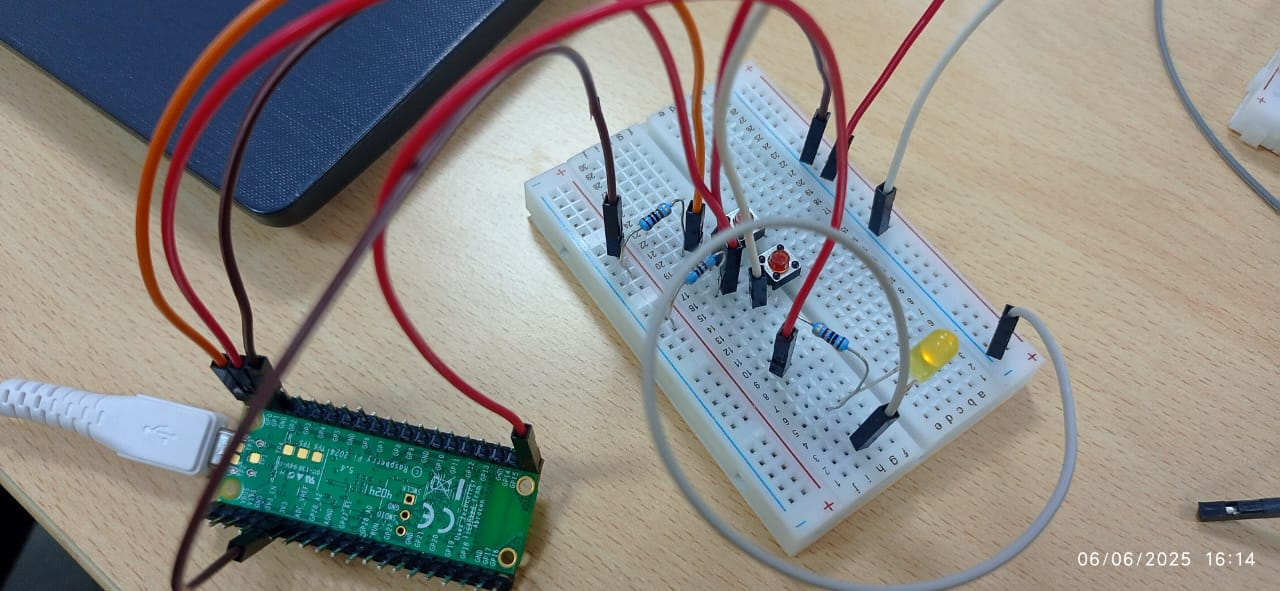
\includegraphics[width=0.95\linewidth]{platformio.jpg}
        \caption*{\textbf{Figure: Implementation of NOR logic circuit}}
\end{figure}
\section*{\textcolor{blue}{Conclusion}}

This question involved a multi-level NOR gate circuit. By simplifying step-by-step and evaluating truth table, we found that the expression simplifies to $\overline{Q + R}$. Hardware implementation verified using Raspberry Pi Pico2W and Arduino Uno confirms the correct logical behavior.

\textbf{Final Answer: (A) $\overline{Q + R}$}

\end{document}
